\documentclass[11pt,a4paper]{article}
\usepackage[english]{babel}
\usepackage[T1]{fontenc}
\usepackage{lmodern}
\usepackage{csquotes}
\usepackage[backend=biber,style=apa]{biblatex}
\addbibresource{references.bib}
\usepackage{graphicx}
\usepackage{booktabs}
\usepackage{siunitx}
\usepackage{amsmath}
\usepackage[hidelinks]{hyperref}
\usepackage[capitalise,noabbrev]{cleveref}

\newcommand{\blackhole}{black hole}
\newcommand{\term}[1]{\textit{#1}}

\setlength{\marginparwidth}{2cm}
\usepackage[disable]{todonotes}

\title{Exploring the Universe: From Stars to Black Holes}
\author{Matej Brnka}
\date{\today}

\begin{document}
\maketitle

\begin{abstract}
This paper provides an introductory overview of the universe, focusing on stars, galaxies, and black holes. It discusses fundamental astronomical concepts, observational methods, and selected physical principles that help explain the structure and evolution of the cosmos.
\end{abstract}

\setcounter{tocdepth}{1}
\tableofcontents

\section{Introduction}
The universe is a vast and fascinating place. In this paper, we explore the mysteries of stars, galaxies, and black holes. Modern astronomy provides powerful tools to investigate the origins, structure, and evolution of the cosmos.

Hawking provides an accessible introduction to the evolution of the universe and the physical principles behind black holes \parencite{hawking1988}.

Black holes are discussed in Section~\ref{sec:black-holes}.

The term \enquote{observable universe} refers to the region from which light has had time to reach an observer.
\section{Stars and Galaxies}
\label{sec:stars-and-galaxies}
\subsection{The Life Cycle of Stars}
Stars are massive celestial objects primarily composed of hydrogen and helium. They generate energy through \textbf{nuclear fusion}. The evolution of a star depends largely on its \textit{initial mass}.

The Sun has a mass of approximately \qty{1.989e30}{\kilogram}. Its effective surface temperature is about \qty{5772}{\kelvin}.

The mass--energy equivalence is expressed as:
\begin{equation}
    E = mc^2
    \label{eq:mass-energy}
\end{equation}

\textcite{carroll2007} describe stellar structure and evolution in detail. Selected properties of stars are summarized in Table~\ref{tab:stellar-properties}.

\begin{table}[htbp]
    \centering
    \caption{Illustrative properties of selected stars}
    \label{tab:stellar-properties}
    \begin{tabular}{lcr}
        \toprule
        Star & Type & Mass ($M_\odot$) \\
        \midrule
        Sun & G-type & 1.0 \\
        Sirius A & A-type & 2.1 \\
        Betelgeuse & Red supergiant & 16.5 \\
        \bottomrule
    \end{tabular}
\end{table}

\subsection{Types of Galaxies}
Galaxies can be classified into several major categories:
\begin{itemize}
    \item Spiral galaxies
    \item Elliptical galaxies
    \item Irregular galaxies
\end{itemize}

The main galaxy categories are illustrated in Figure~\ref{fig:galaxy-types}.

\begin{figure}[htbp]
    \centering
    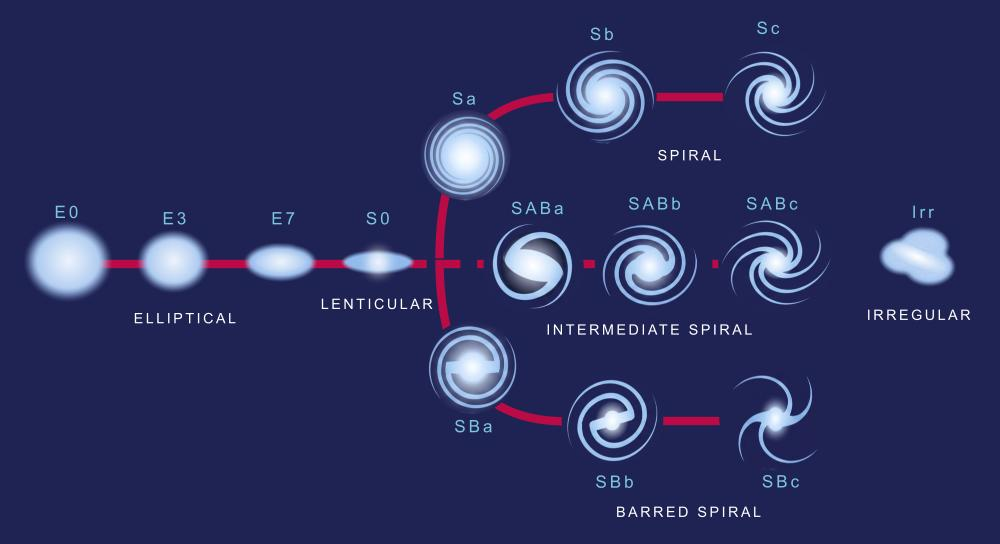
\includegraphics[width=0.8\textwidth]{figures/images/galaxy-types.jpg}
    \caption{Major galaxy morphologies: spiral, elliptical, and irregular.}
    \label{fig:galaxy-types}
\end{figure}

The main morphological categories are summarized in Table~\ref{tab:galaxy-types}.
\begin{table}[htbp]
    \centering
    \caption{Basic galaxy classifications}
    \label{tab:galaxy-types}
    \begin{tabular}{ll}
        \toprule
        Galaxy type & Typical characteristic \\
        \midrule
        Spiral & Disk with spiral arms \\
        Elliptical & Smooth, rounded appearance \\
        Irregular & No regular overall shape \\
        \bottomrule
    \end{tabular}
\end{table}
\section{Black Holes}
\label{sec:black-holes}
\subsection{Formation of Black Holes}
A \blackhole{} can form after the gravitational collapse of a sufficiently massive stellar core.

\subsection{Event Horizons}
The event horizon\footnote{The event horizon is a boundary in spacetime beyond which signals cannot reach a distant observer.} is the boundary beyond which light and other signals cannot escape to distant observers.

The Event Horizon Telescope collaboration published an image of the black hole shadow in the galaxy M87 \parencite{eventhorizon2019}.

The \term{event horizon} is an important concept in general relativity.

\begin{figure}[htbp]
    \centering
    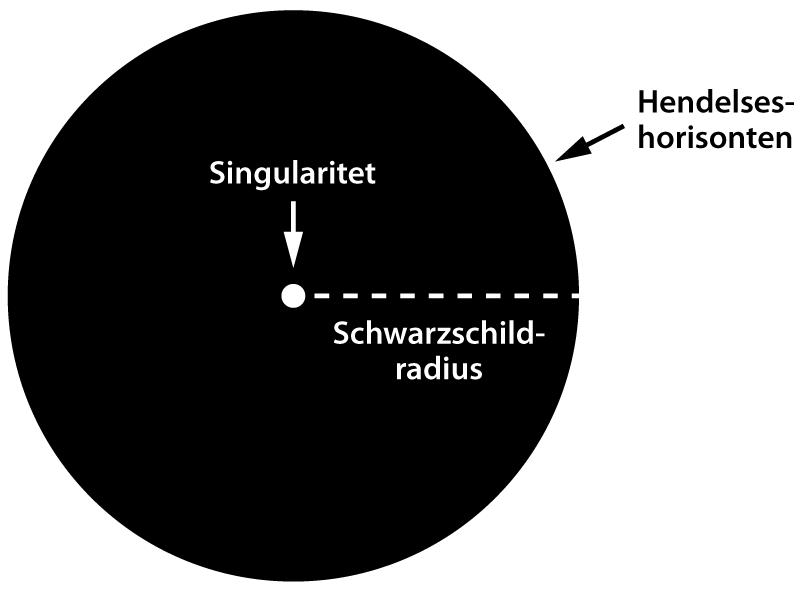
\includegraphics[width=0.75\textwidth]{figures/images/black-hole-diagram.jpg}
    \caption{Simplified schematic of a black hole and its event horizon. Source: Maria Hammerstrøm, SNL (CC BY-NC-SA 3.0). Norwegian labels: singularity, event horizon, Schwarzschild radius.}
    \label{fig:black-hole}
\end{figure}

The Schwarzschild radius is denoted by $r_s$ and depends on the mass $M$ of the object.

The Schwarzschild radius is calculated using Equation~\eqref{eq:schwarzschild-radius}.

\begin{equation}
    r_s = \frac{2GM}{c^2}
    \label{eq:schwarzschild-radius}
\end{equation}
\section{Observing the Universe}
A typical scientific observation process includes:\todo{Add a recent reference about astronomical observations.}
\begin{enumerate}
    \item Collect observational data.
    \item Process and calibrate measurements.
    \item Analyze the results.
    \item Interpret the astronomical findings.
\end{enumerate}

Modern astronomy combines observations, data analysis \& computational models.

Observational data require careful calibration to achieve uncertainties below 1 \% in suitable measurements.

The wavelength $\lambda$ and frequency $\nu$ of electromagnetic radiation satisfy the relation\todo[inline]{Expand this section with a short example of telescope observations.}

\begin{equation}
    \begin{aligned}
        c &= \lambda \nu \\
        \nu &= \frac{c}{\lambda}
    \end{aligned}
    \label{eq:frequency}
\end{equation}
\section{Conclusion}
The study of the universe connects observations with fundamental physical principles. Understanding stars, galaxies, and black holes helps scientists investigate the history and evolution of the cosmos.

Understanding the universe requires combining theoretical models with astronomical observations \parencite{hawking1988,carroll2007}.

\printbibliography

\end{document}